\chapter{Les Ventes (les \'etats des ventes d'articles)}\label{chap:vente}
\index{vente}
\index{\'etats des ventes d'articles}
\index{\'etats des ventes des stocks}

\utilisateurs: \liencaissier, \lienpatron.\\

\chapintro{Ce chapitre d\'ecrit comment consulter
les chiffres d'affaires (les recettes). Le chapitre
explique aussi comment param\'etrer cette
consultation afin d'obtenir des r\'esultats
plus pr\'ecis (ex: le chiffre d'affaire r\'ealis\'e
sur un article).}

\nxsection{Introduction}

\begin{figure}[!htpb]
	\centering
	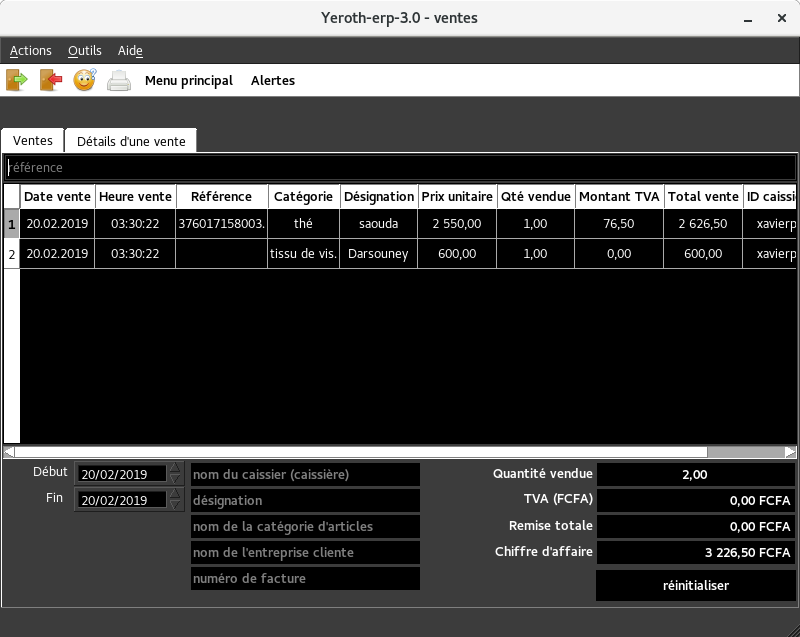
\includegraphics[scale=0.63]{images/yeren-caisse.png}
	\caption{La fen\^etre du module caisse
				(les \'etats de ventes)}~\label{fig:yeren-caisse}
\end{figure}

Le module '\textbf{Caisse}' de \yeren donne une
vue d'ensemble sur toutes les ventes effectu\'ees.
La figure~\ref{fig:yeren-caisse} illustre
l'interface graphique du module '\textbf{Caisse}'.

%-----------------------------------------------------------

\nxsection{Voir le journal des ventes sur une p\'eriode de temps}
\index{consulter le journal des ventes}
\index{voir le journal des ventes}
\index{historique des ventes}

Un utilisateur \textbf{avec le \role \patron} d\'efinit
les dates de d\'ebut et de fin de la p\'eriode sur
laquelle il souhaite voir les ventes. Il peut aussi
ajouter les param\`etres suivants \`a sa requ\^ete:

\begin{enumerate}[1)]
	\item le nom d'un caissier 
		(champs de texte '\textbf{Caissier}')
	\item la d\'esignation d'un l'article
		(champs de texte '\textbf{D\'esignation}')
	\item une cat\'egorie d'articles
		(champs de texte '\textbf{Cat\'egorie}')
	\item le nom d'un client
		(champs de texte '\textbf{Client}')
	\item le num\'ero d'une facture.
		(champs de texte '\textbf{Facture N.}').
\end{enumerate}

Lorsque plus d'un param\`etre est utilis\'e pour la requ\^ete,
\yeren emploi l'op\'erateur logique '\textbf{AND}' pour
g\'en\'erer la requ\^ete.

\textbf{NB:} les utilisateurs \textbf{avec le \role \caissier}
ont seulement acc\`es \`a leur journal des ventes du jour.
Ils ont aussi acc\`es au param\'etrage des \'el\'ements
suivants:

\begin{enumerate}[1)]
	\item la d\'esignation d'un l'article
		(champs de texte '\textbf{D\'esignation}')
	\item une cat\'egorie d'articles
		(champs de texte '\textbf{Cat\'egorie}')
	\item le num\'ero d'une facture.
		(champs de texte '\textbf{Facture N.}').
\end{enumerate}

%-----------------------------------------------------------

\nxsection{Voir les d\'etails d'une vente}
\index{consulter les d\'etails d'une vente}
\index{voir les d\'etails d'une vente}

Il suffit de cliquer deux fois sur la vente s\'electionn\'ee.

%-----------------------------------------------------------

\nxsection{Voir le journal des ventes d'un caissier}
\index{voir le journal des ventes d'un caissier}
\index{voir le chiffre d'affaire r\'ealis\'e avec un caissier}
\index{chiffre d'affaire d'un caissier}

Il suffit de param\'etrer la requ\^ete avec le nom de ce
caissier dans le champs de texte '\textbf{Caissier}' (Voir
la figure~\ref{fig:yeren-caisse}).

%-----------------------------------------------------------

\nxsection{Voir le journal des ventes d'un article}
\index{voir le journal des ventes d'un article}
\index{voir le chiffre d'affaire r\'ealis\'e avec un article}
\index{chiffre d'affaire d'un article}

Il suffit de param\'etrer la requ\^ete avec la d\'esignation
de cet article. Ceci se fait dans le champs de texte
'\textbf{D\'esignation}' (Voir la figure~\ref{fig:yeren-caisse}).

%-----------------------------------------------------------

\nxsection{Voir le journal des ventes d'une cat\'egorie d'articles}
\index{voir le journal des ventes d'une cat\'egorie d'articles}
\index{voir le journal des ventes d'une famille d'articles}
\index{voir le chiffre d'affaire r\'ealis\'e avec une famille d'articles}
\index{chiffre d'affaire d'une cat\'egorie d'articles}

Il suffit de param\'etrer la requ\^ete avec le nom de la
cat\'egorie de cet article. Ceci se fait dans le champs
de texte '\textbf{Cat\'egorie}' (Voir la figure~\ref{fig:yeren-caisse}).

%-----------------------------------------------------------

\nxsection{Voir le journal des achats d'un client nomm\'e}
\index{voir le journal des achats d'un client nomm\'e}
\index{voir le chiffre d'affaire r\'ealis\'e avec un client nomm\'e}

Il suffit de param\'etrer la requ\^ete avec le nom du
client concern\'e. Ceci se fait dans le champs de
texte '\textbf{Client}' (Voir la figure~\ref{fig:yeren-caisse}).

%-----------------------------------------------------------

\nxsection{Voir le journal des ventes d'une facture}
\index{voir les ventes d'une facture}

Il suffit de param\'etrer la requ\^ete avec le num\'ero
de facture correspondant. Ceci se fait dans le champs de
texte '\textbf{Facture N.}' (Voir la figure~\ref{fig:yeren-caisse}).

%-----------------------------------------------------------

\nxsection{Imprimer le journal des ventes au format PDF}
\index{Imprimer le journal des ventes au format PDF}

Il existe deux m\'ethodes pour imprimer 'le journal
des ventes' de la liste des ventes qui appara\^it \`a
la fen\^etre titr\'e '\textbf{Yeren - Caisse}'.

\begin{itemize}[\mycheckmark{purplish}]
	\item \textcolor{purplish}{$\mathbf{1^{\text{\`ere}}}$ \textbf{m\'ethode}}\\
		Cliquer sur le lien '\textbf{Imprimer le journal des
		ventes}' qui se trouve dans le menu
		d\'eroulant '\textbf{Outils}'\\

	\item \textcolor{purplish}{$\mathbf{2^{\text{\`eme}}}$ \textbf{m\'ethode}}\\
		Presser simultan\'ement les boutons \bouton{CTRL}
		et \bouton{P} de votre clavier.
\end{itemize}
